%%%%%%%%%%%%%%%%%%%%%%%%%%%%%%%%%%%%%%

\documentclass[12pt]{article}
%\documentstyle[12pt,psfig,epsf]{article}

\hoffset=-15mm \voffset=-25mm \textwidth=165mm \textheight=245mm
\usepackage{graphicx}
\usepackage{amsmath}
\usepackage{amssymb}
%\usepackage{bigcircle}
\usepackage{wrapfig}
\usepackage{indentfirst}
\usepackage{color}
\usepackage{subfigure}

\begin{document}

\vskip 0.5cm \centerline{\bf\Large What's inside Oleg's code}
\vskip 1cm

\section{Double-differential cross-section of SDD as a function of $M_X^2$ for fixed $t$}
This is similar to what is shown in Fig.8 of~\cite{Jenkovszky11}.
The cross-section reads
$$
\frac{d^2\sigma}{dt dM_X^2}=\frac{1}{(1. - t/0.71)^4} \left(\frac{s}{M_X^2}\right)^{2(1.08 + 0.25t) - 2} \sigma_{PpN}(M_X^2,t) KF(x,t,M_X^2)
$$


$$
\sigma_{PpN}(M_X^2,t)=Im A(M_X^2,t) / m_{proton}
$$

$$
Im A(M_X^2,t) = Im\ \alpha(s) \sum_{i=0}^{2}\frac{1}{(1. - t/0.71)^{4(i+2)}} / ((2*i+2.5-Re\ \alpha(s))^2+im^2)
$$

$$
Im\ \alpha(s) = \sum_{i=0}^{2} s^\delta c_i (1-s_i/s)^(Re\ \alpha(s_i)) \theta(s-s_i) 
$$

$$
c_1=  0.508309,
c_2 = 4.01083,
c_3 = 4558.44.
$$
  
$$
s_1=  1.151,
s_2 = 2.44,
s_3 = 11.7.
$$

Kinematic factor:
$$
KF(x,t,M_X^2) = \frac{x (1-x)^2}{\left(1 - 4m_{proton}^2x^2/t\right)^{1.5}(M_X^2-m_{proton}^2)};
$$

% \begin{figure}[!h]
% \centering
% 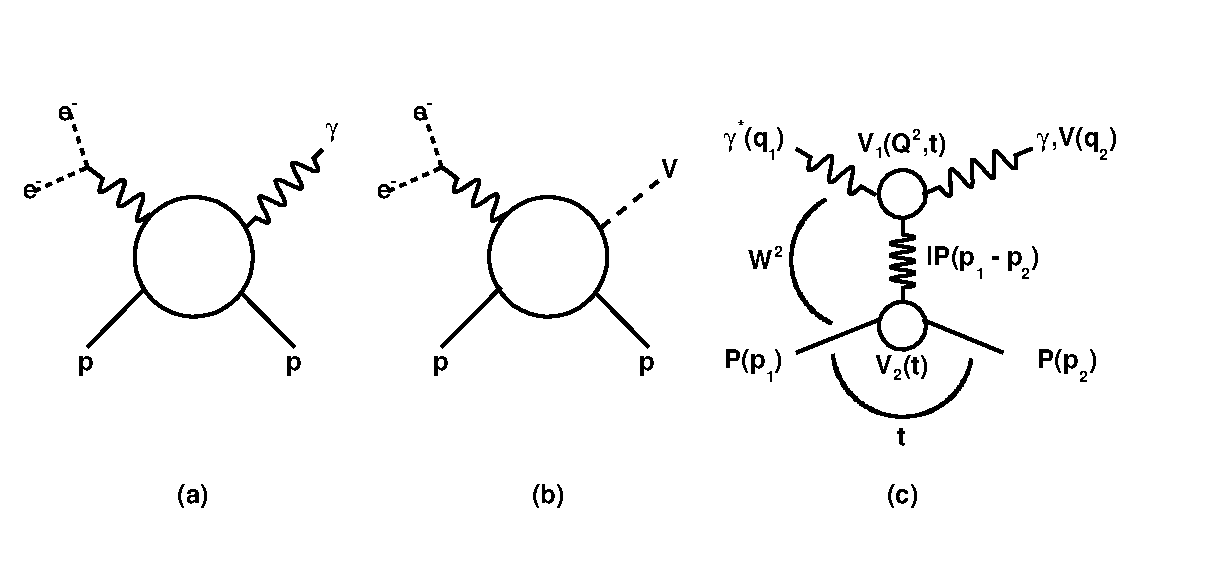
\includegraphics[width=.8\textwidth]{figures/diagrams.eps}
% \caption{Diagrams of DVCS (a) and VMP (b); (c) DVCS (VMP) amplitude in a Regge-factorized form.}
% \label{fig:diagrams}
% \end{figure}

%   $$
%    A(s,t,Q^2,{M_v}^2)= \widetilde{A_s}e^{-i\frac{\pi}{2}\alpha_s(t)}\left(\frac{s}{s_{0}}\right)^{\alpha_s(t)}
%     e^{b_st - n_s\ln{\left(1+\frac{\widetilde{Q^2}}{\widetilde{Q_s^2}}\right)}}
%   $$
%   \begin{equation}
%   +\widetilde{A_h}e^{-i\frac{\pi}{2}\alpha_h(t)}\left(\frac{s}{s_{0}}\right)^{\alpha_h(t)}
%     e^{b_ht - (n_h+1)\ln{\left(1+\frac{\widetilde{Q^2}}{\widetilde{Q_h^2}}\right)}
%     +\ln{\left(\frac{\widetilde{Q^2}}{\widetilde{Q_h^2}}\right)} },
%     \label{eq:Amplitude_FFJS}
%     \end{equation}


\begin{thebibliography}{99}
\bibitem{Jenkovszky11} 1011.0664
\bibitem{Jenkovszky12} 1211.5841
\end{thebibliography}

\end{document}
